\chapter{Modely}

V sekcii \ref{sec:hmm-alignment} sme si zadefinovali HMM pre zarovnávanie sekvenci (obr. \ref{fig:simple-model}).
V našom riešení sme predstavili 2 modifikácie pôvodného HMM na zakomponovanie dodatočnej informácie, pričom sme využili klasifikátory. V oboch modeloch sú klasifikátory rovnaké, aj s rovnakým postupom trénovania. Líši sa len trénovanie samotného HMM a architektúra modelu.

\section{Model s klasifikátorom ako emisiou}

V tomto modeli sme nahradili emisné tabuľky stavov výstupom z klasifikátora.
Model teda bude vyzerať rovnako, aj pravdepodobnosti prechodov zostanú, ale emisná pravdepodobnosť sa nahradí výstupom z klasifikátora.

\begin{figure}[htp]
    \centering
    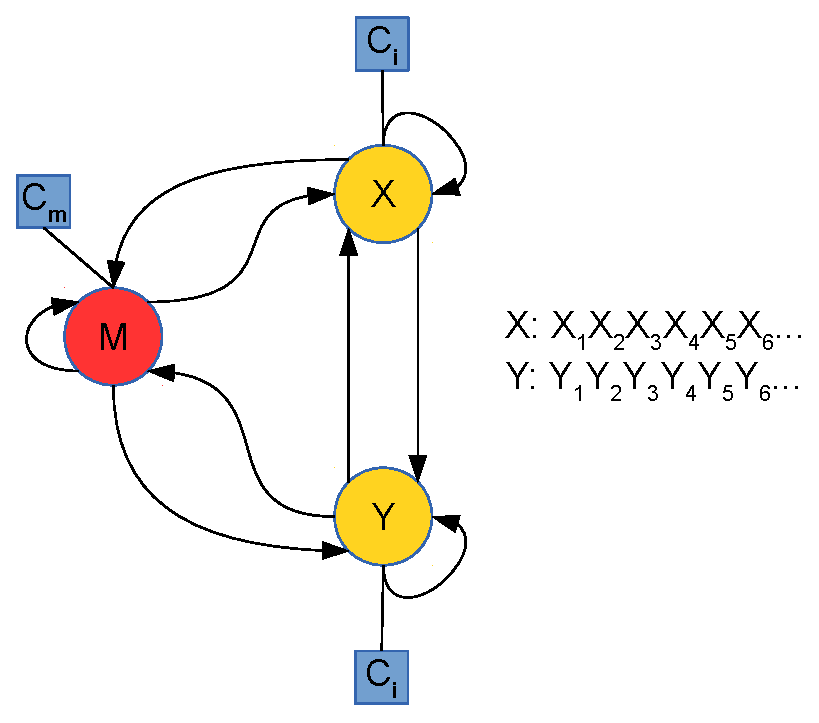
\includegraphics[width=.5\textwidth]{images/model_clf}
    \caption{Model s klasifikátorom ako emisiou}
\end{figure}


Problémom tohto modelu je, že výstup klasifikátora nezodpovedá emisným pravdepodobonstiam, ale akejsi istote klasifikátora o tom, že dve pozície majú byť zarovnané k sebe. Hodnoty z klasifikátora teda nesumujú do 1 a model nie je celkom korektný. V praxi sa však ukázalo, že to až tak nevadí, avšak o takomto modeli už nemóžme hovoriť ako o pravdepodobnostnom. Je len inšpirovaný HMM.1

V tomto modeli sme trénovali iba tranzície, emisie sme mali priamo z natrénovaného klasifikátora.

\section{Model s klasifikátorovou páskou}

Na to aby sme vyriešili problém s korektnosťou predošlého modelu, navrhli sme alternatívny model, ktorý navyše modeluje aj výstup z klasifikátora.
Nemodelujeme teda len dvojicu sekvencií, ale aj sekvenciu výstupov klasifikátora.
Pásku s výstupom z klasifikátora vieme považovať za akýsi hint pre náš zarovnávač.

\begin{figure}[htp]
    \centering
    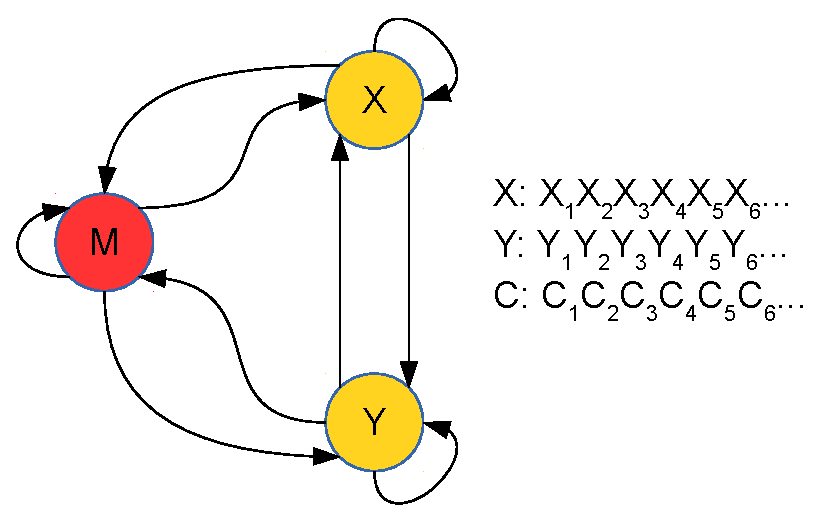
\includegraphics[width=.5\textwidth]{images/model_clf_paska}
    \caption{Model s klasifikátorovou páskou}
\end{figure}


Tento model je síce narozdiel od predošlého korektný pravdepodobnostý model, no má však jednu nevýhodu. Že okrem prípadov, keď klasifikátor vráti hodnotu blízku 0 -- teda tvrdí, že dané 2 pozície by nemali byť zarovnané k sebe (resp. daná pozícia by nemala byť zarovnaná k medzere), penalizuje aj prípady kedy klasifikátor vracia hodnoty blízke 1. Je to z dôvodu, že HMM sa trénuje pomocou frekvenčnej analýzy a pozícií, kde sa vyskytujú hodnoty blízke 1 je menej ako pozícií s hodnotami okolo 0.7.

V tomto modeli sme trénovali aj tranzície aj emisie. Klasifikátorovú pásku sme generovali pomocou oboch klasifikátorov, pričom v Match stave sme použili Match klasifikátor a v Insert stavoch InDel klasifikátor.
Výstupy z klasifikátora sme rozdelili do 10 košov rovnomerne na intervale <0, 1>
